\documentclass[conference]{IEEEtran}
\IEEEoverridecommandlockouts
\usepackage{cite}
\usepackage{amsmath,amssymb,amsfonts}
\usepackage{algorithmic}
\usepackage{graphicx}
\usepackage{textcomp}
\usepackage{xcolor}
\usepackage{booktabs}

\def\BibTeX{{\rm B\kern-.05em{\sc i\kern-.025em b}\kern-.08em
    T\kern-.1667em\lower.7ex\hbox{E}\kern-.125emX}}

\begin{document}

% ============================================================
%  TITLE AND AUTHOR
% ============================================================

\title{Accelerating Lifelong MAPF Optimization via\\
Uncertainty-Based Surrogate-Assisted Evolution Strategies%
\thanks{This thesis was prepared in partial fulfilment of the requirements
for the Degree of Bachelor of Science in Data Science and Artificial
Intelligence, Maastricht University. Supervisor(s): Prof. Gerhard Weiss.}
}

\author{%
  \IEEEauthorblockN{Igor Świerlikowski}
  \IEEEauthorblockA{%
    \textit{Department of Advanced Computing Sciences}\\
    \textit{Faculty of Science and Engineering}\\
    \textit{Maastricht University}\\
    Maastricht, The Netherlands
  }
}

\maketitle

% ============================================================
%  ABSTRACT
% ============================================================

\begin{abstract}
Lifelong Multi-Agent Path Finding (LMAPF) is computationally demanding.
Optimizing guidance graphs with evolutionary algorithms such as CMA-ES
typically requires hundreds of thousands of expensive multi-agent
simulations. This paper introduces an uncertainty-aware surrogate-assisted
approach that replaces the majority of those simulations with predictions
from an ensemble of Multi-Layer Perceptrons. An Upper Confidence Bound
(UCB) selection mechanism balances exploitation of high-predicted-fitness
candidates with exploration of uncertain search-space regions, preventing
surrogate exploitation as the CMA-ES distribution shifts into unexplored
regions during evolution. The surrogate reaches the same throughput quality
as the full-budget baseline using 2.81--2.92x fewer simulations across two
random seeds (49k vs.\ 137k simulations to first reach the same throughput
threshold on the primary run). A gradient refinement experiment provides direct evidence of surrogate
exploitation and confirms that the conservative UCB design guards against it.
A diagnostic analysis using full-leakage, oracle, and noise-bound tests
identifies high inter-emitter population diversity, quantified as
intraclass correlation (ICC), as a necessary condition for surrogate
effectiveness. A single-emitter baseline without any surrogate reaches
the same quality threshold at 3.30x fewer simulations than the vanilla
multi-emitter run, confirming that emitter focusing rather than surrogate
ranking is the primary efficiency mechanism.
\end{abstract}

\begin{IEEEkeywords}
lifelong multi-agent path finding, surrogate-assisted optimization,
CMA-ES, uncertainty quantification, Upper Confidence Bound, evolutionary computation,
intraclass correlation
\end{IEEEkeywords}


% ============================================================
%  1. INTRODUCTION
% ============================================================

\section{Introduction}

Lifelong Multi-Agent Path Finding is central to modern automated logistics.
It manages the robot fleets in fulfillment centers such as those operated
by Amazon and Ocado. Unlike traditional path finding, where agents stop
after reaching a single destination, LMAPF is a continuous process: agents
receive new goals immediately upon completing their current task. The
standard approach to this problem is Guidance Graph Optimization (GGO),
introduced by Zhang et al.~\cite{zhang2024}, in which a Covariance Matrix
Adaptation Evolution Strategy (CMA-ES) learns a set of flow weights that
overlay the warehouse map. These weights guide decentralized agents toward
high-throughput routes and reduce congestion.

A key bottleneck limits the scalability of GGO. To evaluate a single
candidate set of flow weights, the optimizer must run multiple complete
multi-agent simulations, each requiring hundreds of timesteps to produce a
stable throughput measurement. A standard 300-generation run requires
150,000 simulations and roughly 9.5 hours of wall-clock time on an 8-core
machine. This makes the method too slow for dynamic environments where
warehouse layouts or goal distributions change frequently, and limits the
number of configurations that can be tested during initial deployment.
The online extension of GGO explicitly identifies surrogate-assisted
optimization as a direction for future work~\cite{zang2025}.

This paper addresses the problem by integrating a machine learning
surrogate into the CMA-ES loop. The surrogate is trained on observed
(solution, throughput) pairs and used to pre-screen candidate solutions
before simulation. Only the most promising candidates and those in
unexplored regions are passed to the simulator. Three research questions
guide the work. First, how can a surrogate model be integrated into the
CMA-ES framework for LMAPF throughput prediction? Second, how much does
surrogate-assisted pre-screening reduce computation time relative to the
baseline? Third, how does uncertainty tracking affect surrogate stability
and prevent exploitation compared to a point-estimate model?
Beyond these questions, the analysis examines what structural conditions
make surrogate pre-screening feasible at all, identifying population
diversity as a necessary precondition whose absence renders any surrogate
ineffective regardless of model capacity.

The main contributions are as follows. We show that an ensemble of
bootstrapped MLPs achieves a Spearman rank correlation of 0.78--0.94 in a
realistic sliding-window test, sufficient for effective pre-screening.
The surrogate reaches equivalent throughput to the vanilla baseline
using 2.81x fewer simulations (49k vs.\ 137k simulations to first reach
$\tau = 8.23$). A gradient
refinement experiment predicted a $+$0.95 throughput gain but measured a
$-$0.11 decrease in real simulation, giving direct evidence of surrogate
exploitation. Finally, we extend the framework to the online GGO setting
of Zang et al.~\cite{zang2025}. The surrogate reduces the required
simulations from 10,000 to 3,520 in the online setting, a 2.84x
reduction, reaching equivalent throughput quality at a 2.41x crossover
speedup.


% ============================================================
%  2. BACKGROUND AND RELATED WORK
% ============================================================

\section{Background and Related Work}

\subsection{Guidance Graph Optimization}

Zhang et al.~\cite{zhang2024} introduced an automated method for
generating traffic rules for robot warehouses. Given a warehouse floor plan
as a graph $G = (V, E)$, the optimization assigns a scalar flow weight
$w_e \in \mathbb{R}$ to each directed edge $e \in E$. A decentralized
pathfinding planner uses these weights as directional biases. Throughput
$\tau$ measures the mean number of tasks completed per timestep at steady
state, averaged over a fixed number of agents and simulation steps. The
baseline optimizer uses CMA-ES~\cite{hansen2016} with multiple
independent emitters~\cite{fontaine2020}. Each emitter maintains a
multivariate normal distribution over the weight space; at each generation
it proposes 20 candidate solutions, evaluates their throughput, and
updates its distribution parameters to move toward higher-throughput
regions.

\subsection{Surrogate-Assisted Evolutionary Computation}

Surrogate-assisted evolutionary computation reduces the number of expensive
fitness evaluations by replacing some with predictions from a cheaper
model. The standard approach evaluates only a subset of each generation
using the true fitness function and fills the rest with surrogate
predictions~\cite{jin2011}. A known problem with this strategy is surrogate
exploitation: the optimizer finds regions where the model overestimates
fitness and the search is directed away from genuine improvements.

Uncertainty quantification offers a way to address this. By measuring
model confidence, the algorithm can balance exploiting high-predicted-fitness
regions against exploring uncertain ones. The Upper Confidence Bound
criterion, from the multi-armed bandit literature~\cite{auer2002}, captures
this trade-off as a single scalar score and has been applied to Bayesian
optimization and surrogate-assisted search~\cite{shahriari2016}. This work
applies it to multi-emitter CMA-ES, where natural distribution shifts
during evolution move the search into unexplored regions and exploration
matters most. Zang et al.~\cite{zang2025} extend the GGO
framework to an online setting, optimizing a CNN policy that adapts edge
weights in real time based on observed traffic. Their paper explicitly
suggests surrogate-assisted optimization as a direction for future work,
which this paper addresses in Section~\ref{sec:online}.


% ============================================================
%  3. PROBLEM DEFINITION
% ============================================================

% ============================================================
%  4. METHODOLOGY
% ============================================================

\section{Methodology}

\subsection{Infrastructure and Baseline}

The warehouse environment is represented as a directed graph where each
edge carries a flow weight; the full weight vector $\mathbf{w} \in
\mathbb{R}^{|E|}$ is the parameter optimized by CMA-ES, with $|E| =
4{,}074$ (948 wait weights and 3,126 directed edge weights on the warehouse
map). Throughput $\tau(\mathbf{w})$ is the mean number of tasks completed
per timestep, averaged over $S = 5$ simulation seeds and $T = 1{,}000$
timesteps per seed; $S$ is increased to 100 for final robustness
comparisons. Because each evaluation requires a full multi-agent
simulation, $\tau$ is the main computational bottleneck.

The optimization pipeline consists of a Python wrapper around a C++ LMAPF
simulator running inside a Docker container. Multiprocessing across 8
workers gives a 2.1$\times$ speedup, reducing per-generation wall-clock
time from roughly 5 minutes to roughly 2 minutes. The baseline uses a
multi-emitter CMA-ES with 5 emitters, each proposing 20 candidates, giving
100 candidates per generation. Over 300 generations this totals 150,000
simulations (100 candidates $\times$ 5 seeds $\times$ 300 generations) and
roughly 9.5 hours of wall-clock time.

\subsection{Surrogate Architecture Selection}
\label{sec:feasibility}

We ran an offline feasibility study comparing XGBoost, Convolutional
Neural Networks (CNN), and Multi-Layer Perceptrons (MLP) using a
sliding-window temporal test: the model is trained on generations
$[0, g)$ and tested on generation $g$ across 8 test points, matching
the live-loop condition. XGBoost matched MLP accuracy but required
100--250 seconds per training run, comparable to a full-evaluation
generation, which would cancel out pre-screening savings. The CNN showed
no consistent benefit from spatial representation of the weight vector
($\rho$ as low as 0.05 at generation 10). The MLP was therefore selected;
its three-layer (256-128-64) architecture provides sufficient capacity at
the 2,000--20,000 sample range of this setting, with model weights kept
between generations and incremental fine-tuning on 100 new samples taking
only 2--5 seconds.

\subsection{Surrogate-Assisted CMA-ES Loop}

The surrogate-assisted pipeline replaces a fraction of full evaluations
with model predictions each generation. The loop runs in three modes,
shown in Fig.~\ref{fig:architecture}.


\begin{figure}[htbp]
  \centerline{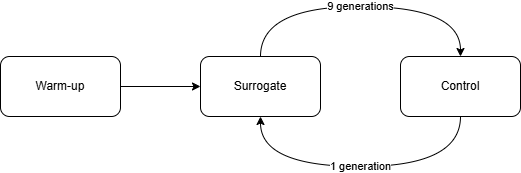
\includegraphics[width=0.48\textwidth]{fig2_flowchart}}
  \caption{The three-phase surrogate-assisted CMA-ES loop. The Surrogate
           Phase uses the UCB score $\text{score} = \mu + \lambda\sigma$
           to select which of the 100 CMA-ES proposals receive full
           simulation.}
  \label{fig:architecture}
\end{figure}

During the \emph{Warmup Phase} (generations 0--19), all 100 candidates
receive full simulation to collect 2,000 training points before any
pre-screening begins. Twenty warmup generations provide roughly double the
minimum data volume at which the offline ensemble achieves reliable rank
correlation (Section~\ref{sec:feasibility}), ensuring pre-screening does
not begin on an undertrained model.
During the \emph{Evolution Control Phase},
triggered every 10 generations, all candidates again receive full
evaluation and the ensemble is retrained on the full history to prevent
the model from going stale as the CMA-ES distribution shifts. The
10-generation interval limits full-evaluation overhead to roughly 10\%
of the simulation budget while providing a regular model refresh.
During the
\emph{Surrogate Phase}, which covers most generations, the ensemble
scores all 100 proposals and the top 20 by score are sent to the simulator.
Surrogate predictions for the remaining 80 candidates are passed to the
CMA-ES update as placeholder fitness values, and the ensemble is fine-tuned
on the 20 new (solution, throughput) pairs. The 20-candidate limit targets
a theoretical 5x speedup and is justified by the population structure: at
ICC near 0.95 the surrogate reliably identifies which emitter a candidate
belongs to, making it effective at separating the top proposals from the
rest.

\subsection{Ensemble UCB Acquisition Function}

To estimate prediction uncertainty, we train 5 bootstrapped MLP instances
on independently resampled subsets of the training data. Five members
follows established practice for bootstrap ensembles in surrogate-assisted
optimization~\cite{lakshminarayanan2017}, giving stable
disagreement estimates without disproportionate training overhead. For a candidate
solution $\mathbf{w}$, each model $f_k$ produces a throughput prediction
$\hat{\tau}_k(\mathbf{w})$. The ensemble mean and standard deviation are:
\begin{align}
  \mu(\mathbf{w}) &= \frac{1}{5} \sum_{k=1}^{5} \hat{\tau}_k(\mathbf{w}),
  \label{eq:mu} \\
  \sigma(\mathbf{w}) &= \sqrt{\frac{1}{5} \sum_{k=1}^{5}
    \bigl(\hat{\tau}_k(\mathbf{w}) - \mu(\mathbf{w})\bigr)^2}.
  \label{eq:sigma}
\end{align}
The UCB score used for candidate selection is:
\begin{equation}
  \text{score}(\mathbf{w}) = \mu(\mathbf{w}) + \lambda \cdot \sigma(\mathbf{w}),
  \label{eq:ucb}
\end{equation}
where $\lambda \geq 0$ controls the exploration weight. At $\lambda = 0$,
candidates are ranked by mean prediction alone. As $\lambda$ increases,
candidates in regions with high ensemble disagreement receive a score
boost and are prioritized for simulation. We test $\lambda \in
\{0, 1.0, 2.0\}$ in Section~\ref{sec:results}; the ablation selects
$\lambda = 1.0$ as the final value.

This interacts directly with the natural distribution shifts that occur
during CMA-ES evolution. As the population moves through the
$|E|$-dimensional weight space, the ensemble regularly encounters
candidate regions it has not previously seen, and ensemble disagreement
$\sigma$ is large for those candidates. The UCB score then promotes them
for simulation regardless of their mean prediction. Once the ensemble
collects training data for the new region, $\sigma$ drops over the next
few control generations. In well-explored regions $\sigma \approx 0$,
so the UCB score reduces to the mean prediction.


% ============================================================
%  5. EXPERIMENTAL SETUP
% ============================================================

\section{Experimental Setup}

The 300-generation budget, 5-emitter configuration, and 20-candidates-per-emitter
structure follow Zhang et al.~\cite{zhang2024} to ensure a comparable baseline.
The baseline ran for 300 generations, evaluating 100 candidates over 5
seeds, totaling 150,000 simulation runs and roughly 9.5 hours of wall-clock
time. All surrogate-assisted configurations used the same 300-generation
span and the same 5-seed evaluation for candidates that received full
simulation, giving 49,200 simulation runs in total (9,840 unique candidate
evaluations against 30,000 for the baseline).

Performance is measured by final throughput, total simulation count, and
wall-clock time. All throughput values reported here are from a
100-simulation robustness test run on the best solution found by each
method. The 5-simulation training scores are affected by seed variance;
correcting to 100-simulation means reduces this noise and gives a fair
basis for comparison.

The primary comparison uses throughput versus cumulative simulation count
rather than throughput versus generation index. Surrogate generations use
around 164 simulations while full-evaluation generations use 500, so a
generation-by-generation plot conflates efficiency with training progress.

Four configurations are compared: (i) Vanilla CMA-ES (full budget
baseline), (ii) Surrogate V1 (point-estimate MLP, $\lambda = 0$),
(iii) Surrogate V3 (ensemble UCB, $\lambda = 1.0$; V2 was an intermediate
configuration not included in the final comparison), and (iv) an ablation
with $\lambda = 2.0$. All surrogate configurations use 49,200 simulation
runs.

\subsection{Online GGO Extension}
\label{sec:online_setup}

To test whether the surrogate framework transfers beyond static edge
weights, we apply it to the online GGO setting of Zang et
al.~\cite{zang2025}. Here the search space is the 4,271-parameter space
of a CNN guidance policy. Unlike static edge weight vectors, raw CNN
parameters have no direct spatial interpretation, making them
significantly harder for the surrogate to model. Each evaluation chains
50 sequential simulator calls, making it roughly 3.8$\times$ slower per
generation than the offline case (460 s vs.\ 120 s).

The online vanilla baseline ran for 100 generations with $n_\text{evals} =
1$ seed per candidate, totaling 10,000 simulation runs and 13.8 hours of
wall-clock time. The surrogate-assisted run used the same three-phase loop
with a warmup of 10 generations bootstrapped from vanilla data to avoid
redundant re-simulation, giving 3,520 total simulation runs and 4.9 hours
of wall-clock time.


\subsection{Robustness Experiments}
\label{sec:robustness_setup}

To assess whether the results generalize beyond the primary configuration,
two additional experiments were run using the same hyperparameters as the
main offline study. First, the vanilla vs.\ V3 comparison was repeated on
the warehouse map with a different random seed (seed 123) to test seed
sensitivity. Second, both methods were applied to a structurally different
map (random-32x32, a 32$\times$32 random grid, seed 42) to assess
generalization to a different environment. For both additional runs,
throughput values are corrected to 100-simulation means.

% ============================================================
%  6. RESULTS
% ============================================================

\section{Results}
\label{sec:results}

\subsection{Baseline Convergence}

The vanilla CMA-ES run improves quickly early on and then slows. Mean
population throughput rose from 3.57 at generation 0 to 7.13 at
generation 100, 8.05 at generation 200, and roughly 8.29 at generation
300. The curve was clearly flattening by generation 250, gaining only
$+0.10$ over the last 50 generations. The occasional step increases
visible in the convergence curve are consistent with the natural dynamics
of multi-emitter CMA-ES as individual emitters converge and populations
shift.

\begin{figure}[htbp]
  \centerline{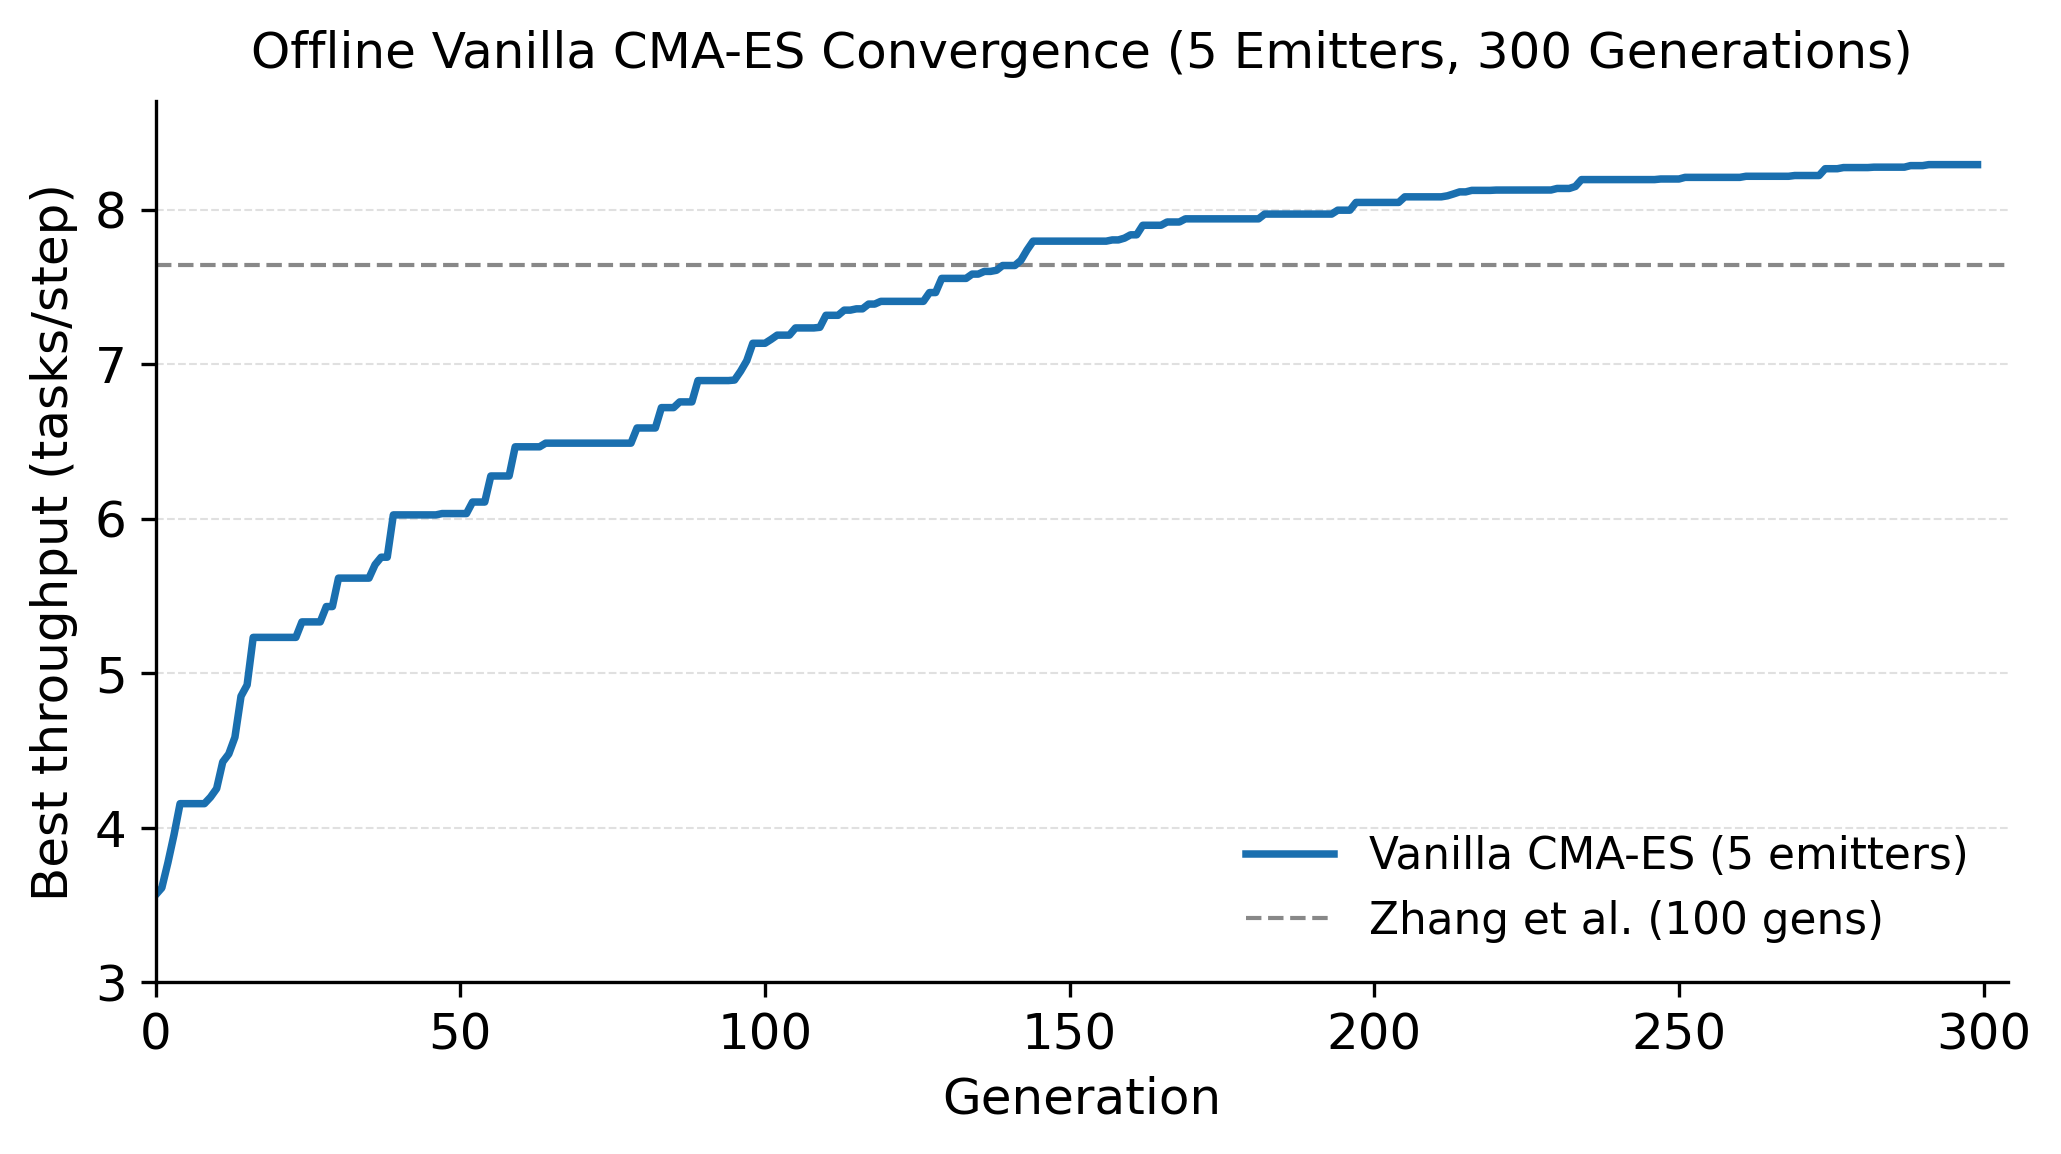
\includegraphics[width=0.48\textwidth]{fig3_baseline_convergence}}
  \caption{Baseline CMA-ES convergence. The dashed line shows the throughput
           reported by Zhang et al.~\cite{zhang2024} for a 100-generation run,
           which our 300-generation run surpasses at generation~145.}
  \label{fig:baseline}
\end{figure}

\subsection{Main Comparison}

Fig.~\ref{fig:efficiency} shows the sample efficiency comparison. The
primary metric is crossover speedup: the number of simulations each method
needs to first reach a matched throughput quality of $\tau = 8.23$. Vanilla
CMA-ES reaches this threshold at generation 274, corresponding to 137,000
simulations. Surrogate V3 reaches the same threshold at generation 297,
using only 49,000 simulations. This gives a crossover speedup of
\textbf{2.81x}. The V3 run completed in 12,539 seconds (3.5 hours),
compared to roughly 9.5 hours for vanilla, a 2.71x wall-clock reduction;
the slight excess over the simulation-count ratio reflects fixed surrogate
training and inference overhead. Vanilla CMA-ES ran for 300 generations. V3 ran for 400
generations in total; at generation 300 its score is comparable to
vanilla's, and by generation 400 it reaches 8.33, confirming the surrogate
does not degrade solution quality over a longer run.

Table~\ref{tab:results} compares all configurations at an equal simulation
budget of $\approx$49k simulations. At this budget, vanilla CMA-ES has
completed roughly 98 generations and reached a corrected throughput of
7.0198. Vanilla reaches only generation~98 because it evaluates 100 candidates
per generation over 5 seeds (500 simulation runs); the surrogate screens most
candidates and runs roughly 164 real simulations per generation, so the
same budget covers the full 300-generation schedule. The generation gap is
the mechanism of the quality improvement, not a confound. All three surrogate
configurations achieve substantially higher quality within the same budget.
Same budget improvements are reported in Table~\ref{tab:results}.

\begin{table}[htbp]
  \caption{Matched-Budget Quality Comparison ($\approx$49k simulations each).
           Vanilla is evaluated at its best solution found by generation~98;
           surrogate methods run their full 300-generation schedule within
           the same budget. All values are 100-simulation corrected means.}
  \label{tab:results}
  \begin{center}
    \begin{tabular}{lccc}
      \toprule
      \textbf{Method} & \textbf{Throughput} & \textbf{95\% CI} & \textbf{vs.\ Vanilla} \\
      \midrule
      Vanilla CMA-ES (gen $\approx$98)          & 7.0198 & [7.00, 7.04] & N/A            \\
      V1 (point-estimate, $\lambda=0$)            & 8.0385 & [8.02, 8.05] & $+$14.5\%      \\
      Ablation ($\lambda=2.0$)                    & 7.8594 & [7.85, 7.87] & $+$12.0\%      \\
      \textbf{V3 (ensemble, $\lambda=1.0$)}   & \textbf{8.1523} & \textbf{[8.14, 8.17]} & $\mathbf{+16.1\%}$ \\
      \bottomrule
    \end{tabular}
  \end{center}
\end{table}

\subsection{Robustness Across Seeds and Maps}
\label{sec:robustness}

Table~\ref{tab:robustness} reports the crossover-point speedup across all
four experimental conditions.

Seed~123 yields a 2.92x speedup (Table~\ref{tab:robustness}), consistent
with the seed-42 result and confirming the speedup is not attributable to
a fortunate draw. In both warehouse conditions the surrogate's 100-sim
corrected quality also exceeds vanilla's: $+0.084$ at seed~42 and
$+0.033$ at seed~123.

On the random-32x32 map the surrogate achieves higher final quality than
vanilla, but the crossover speedup is \textbf{1.00x}. Because the warmup phase runs full evaluations
on both methods using the same seed, the first 20 generations are
identical. This map is comparatively simple: both methods reach the quality
target well before the warmup phase ends and the surrogate begins screening
candidates. On problems that converge this quickly there is no real
opportunity for surrogate pre-screening to provide a speedup.

\begin{table}[htbp]
  \caption{Crossover-Point Speedup Across All Experimental Conditions}
  \label{tab:robustness}
  \begin{center}
    \begin{tabular}{llcc}
      \toprule
      \textbf{Condition} & \textbf{Setting} & \textbf{$\tau$ (vanilla)} & \textbf{Speedup} \\
      \midrule
      Warehouse seed~42  & Offline & 8.2205 & \textbf{2.81x} \\
      Warehouse seed~123 & Offline & 8.0176 & \textbf{2.92x} \\
      Online GGO         & Online  & 7.433  & \textbf{2.41x} \\
      Random-32x32 s42   & Offline & 3.3642 & \textbf{1.00x}$^{\dagger}$ \\
      \bottomrule
      \multicolumn{4}{l}{$^{\dagger}$Converges before surrogate phase activates; see text.}
    \end{tabular}
  \end{center}
\end{table}

\begin{figure}[htbp]
  \centerline{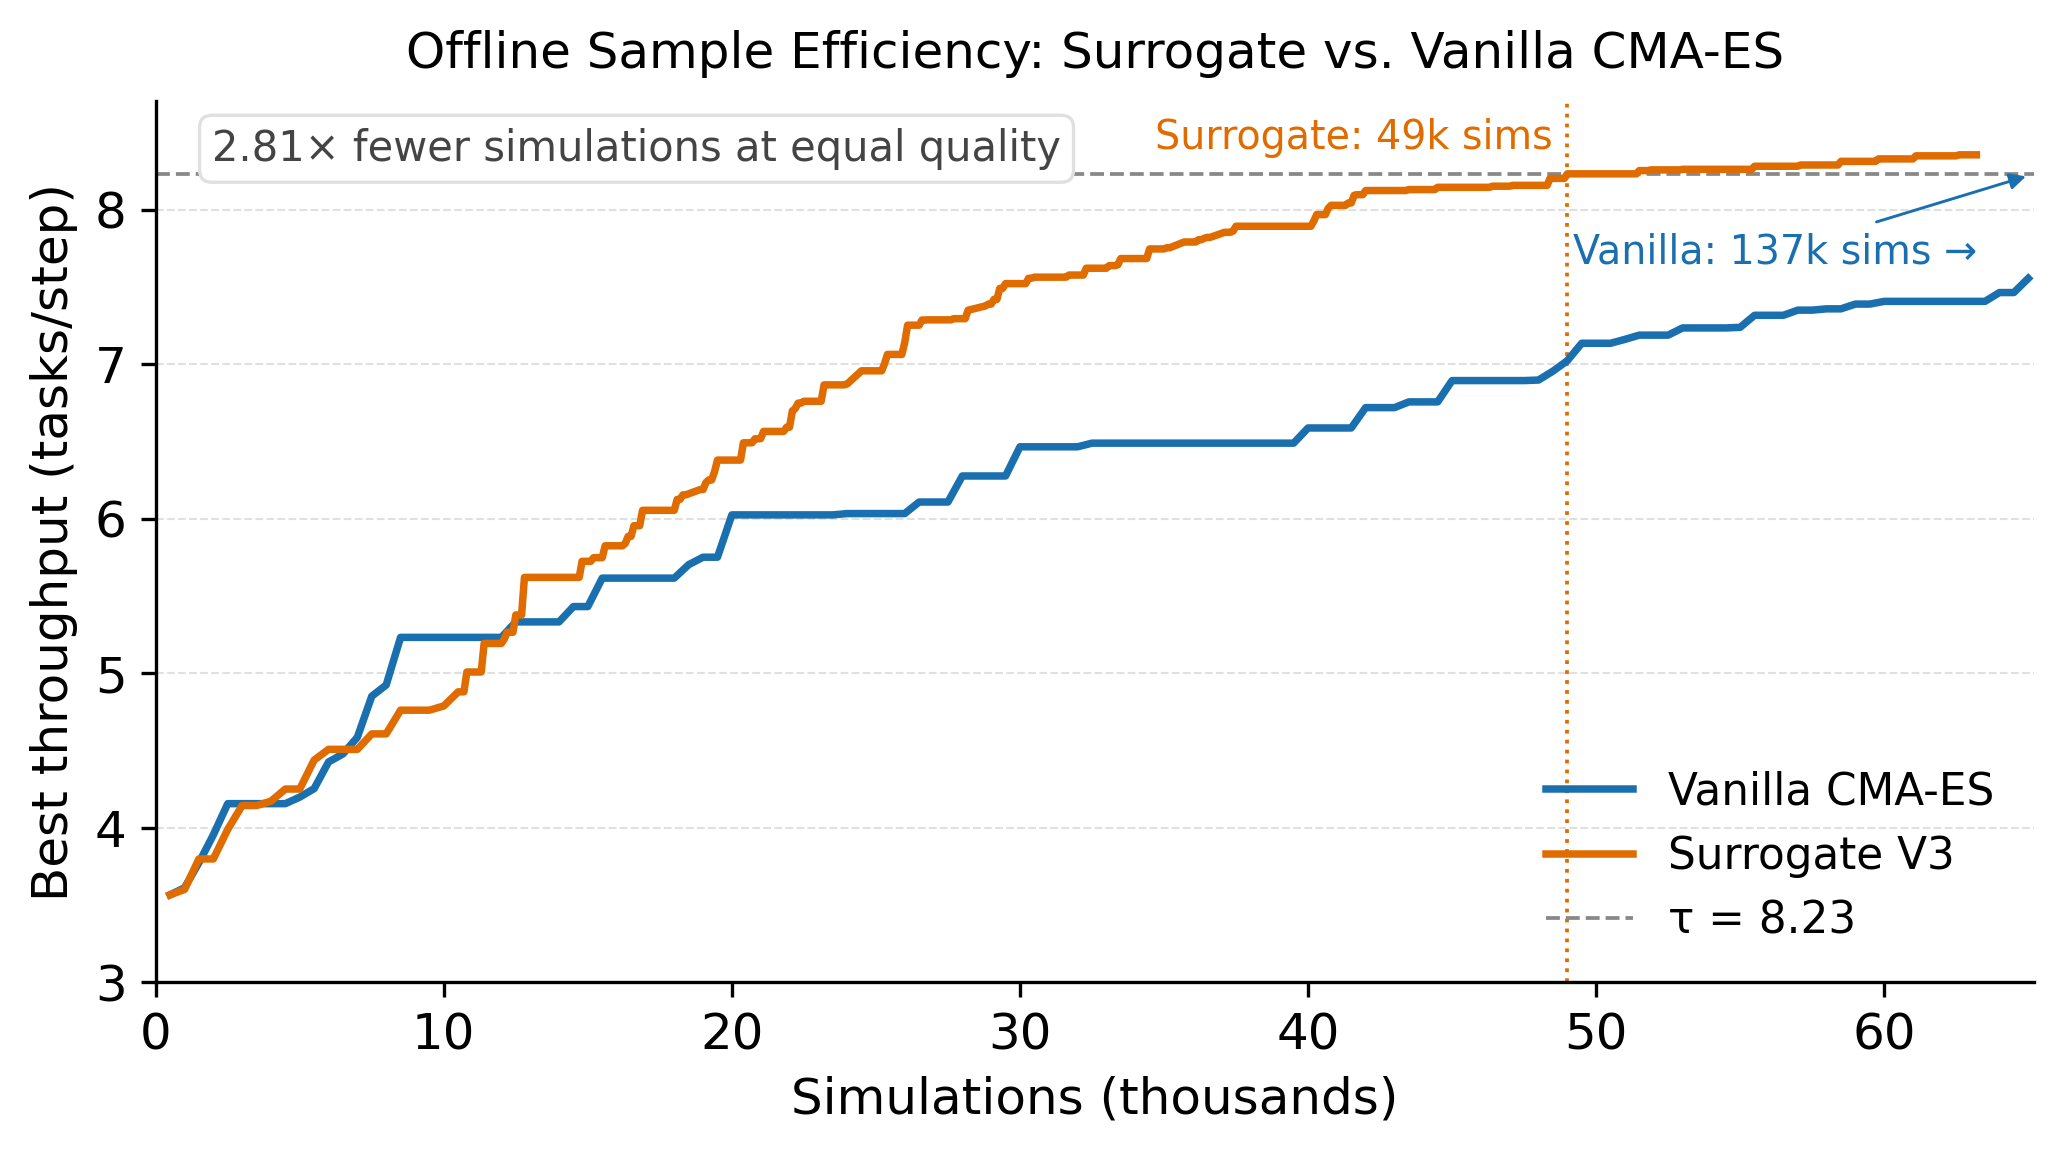
\includegraphics[width=0.48\textwidth]{fig4_sample_efficiency}}
  \caption{Sample efficiency: best throughput vs.\ cumulative simulations.
           Both methods run 300 generations. The surrogate uses roughly
           164 real simulations per generation vs.\ 500 for vanilla, so
           slower per-generation progress is expected. Both reach
           $\tau = 8.23$; the surrogate does so at 49k simulations
           against 137k for vanilla, a 2.81x crossover speedup.}
  \label{fig:efficiency}
\end{figure}

\subsection{Surrogate Accuracy in the Live Loop}

The mean Spearman $\rho$ in the live surrogate loop was 0.49, below the
0.78--0.94 range from the offline feasibility study. Three factors explain
this. First, warmup generations (0--19) produce low-$\rho$ measurements
(0.10--0.50) before enough training data has accumulated. Second, as the
CMA-ES distribution shifts into new regions of the weight space, $\rho$
temporarily drops to 0.22--0.38 at the first control generation after the
shift, because the model has no data for those regions. Third, surrogate
generations add only 20 real evaluations each instead of the 100 assumed
in the offline study, so training data grows five times more slowly. When
warmup and immediate post-shift generations are excluded, $\rho$ generally
ranges 0.40--1.0, consistent with the feasibility study results and
sufficient for effective rank-based pre-screening in the multi-emitter
setting, where the dominant task is identifying which emitter a candidate
belongs to rather than fine-grained ranking within a single distribution
(see Section~\ref{sec:population_structure}).

\subsection{Diagnosing the Source of Surrogate Rank Correlation}
\label{sec:population_structure}

The stable-phase rank correlation of 0.40--1.0 confirms that the
surrogate provides a useful signal, but it does not reveal what that
signal is. A surrogate could achieve high $\rho$ either by learning the
fitness landscape (ranking candidates by intrinsic quality within an
emitter's distribution) or by exploiting structural features of the
population (identifying which emitter a candidate belongs to). To
distinguish these cases, we ran three escalating diagnostic tests on a
single-emitter baseline (1 emitter, popsize $= 100$, 100 generations;
same map and seed as the main run), where the second explanation cannot
apply by construction.

Test 1: Model capacity (full-leakage).
Each model was trained on all 100 candidates from generation $g$ and
immediately evaluated on those same 100 candidates.
XGBoost achieved $\rho = 0.999$--$1.000$ across all test generations,
confirming that it can perfectly memorise and rank data it has seen.
MLP achieved $\rho = 0.79$--$0.89$ under regularisation.
Model capacity is \emph{not} the bottleneck.

Test 2: Temporal distribution shift (oracle).
Each model was trained on a random 80-candidate subset of generation $g$
and evaluated on the remaining 20 candidates from the \emph{same}
generation, eliminating any temporal gap.
Both models produced $\rho \approx 0$ (XGBoost mean $= +0.03$;
MLP mean $= -0.03$), despite perfect in-sample ranking.
Distribution shift is \emph{not} the bottleneck.

Test 3: Measurement noise.
Given population and seed-variance estimates, the theoretical
rank-correlation ceiling is $\rho \leq 0.99$, ruling out measurement
noise as the bottleneck~\cite{spearman1904}.

The only remaining explanation is local landscape roughness:
the throughput function is non-smooth at the scale of within-generation
variation, so knowing the quality of 80 nearby solutions provides
essentially no information about 20 others drawn from the same
CMA-ES distribution.

This raises the question of why the surrogate works in the five-emitter
setting at all.
We adapt the intraclass correlation coefficient from psychometrics~\cite{shrout1979}
to quantify population structure in the multi-emitter setting:
\begin{equation}
  \text{ICC} = \frac{\sigma^2_\text{between}}
    {\sigma^2_\text{between} + \sigma^2_\text{within}},
  \label{eq:icc}
\end{equation}
where $\sigma^2_\text{between}$ is the variance of per-emitter mean
throughputs and $\sigma^2_\text{within}$ is the mean within-emitter
variance. This corresponds to the ICC(1,1) variant of Shrout and
Fleiss~\cite{shrout1979} (one-way random effects, single measures).
A high ICC means most population diversity comes from between-emitter
differences, making the surrogate's effective task \emph{cluster
identification} rather than fine-grained regression.

Fig.~\ref{fig:rho_emitter} (top panel) shows per-emitter throughput at
evolution control generations of the surrogate run: emitter~2 diverges
to 8.22 while emitters 0, 1, 3, and 4 plateau near 5.1 from generation
60 onwards, producing the between-emitter variance that drives ICC
growth. The bottom panel compares ICC trajectories from the vanilla and
surrogate runs.

\begin{figure}[htbp]
  \centerline{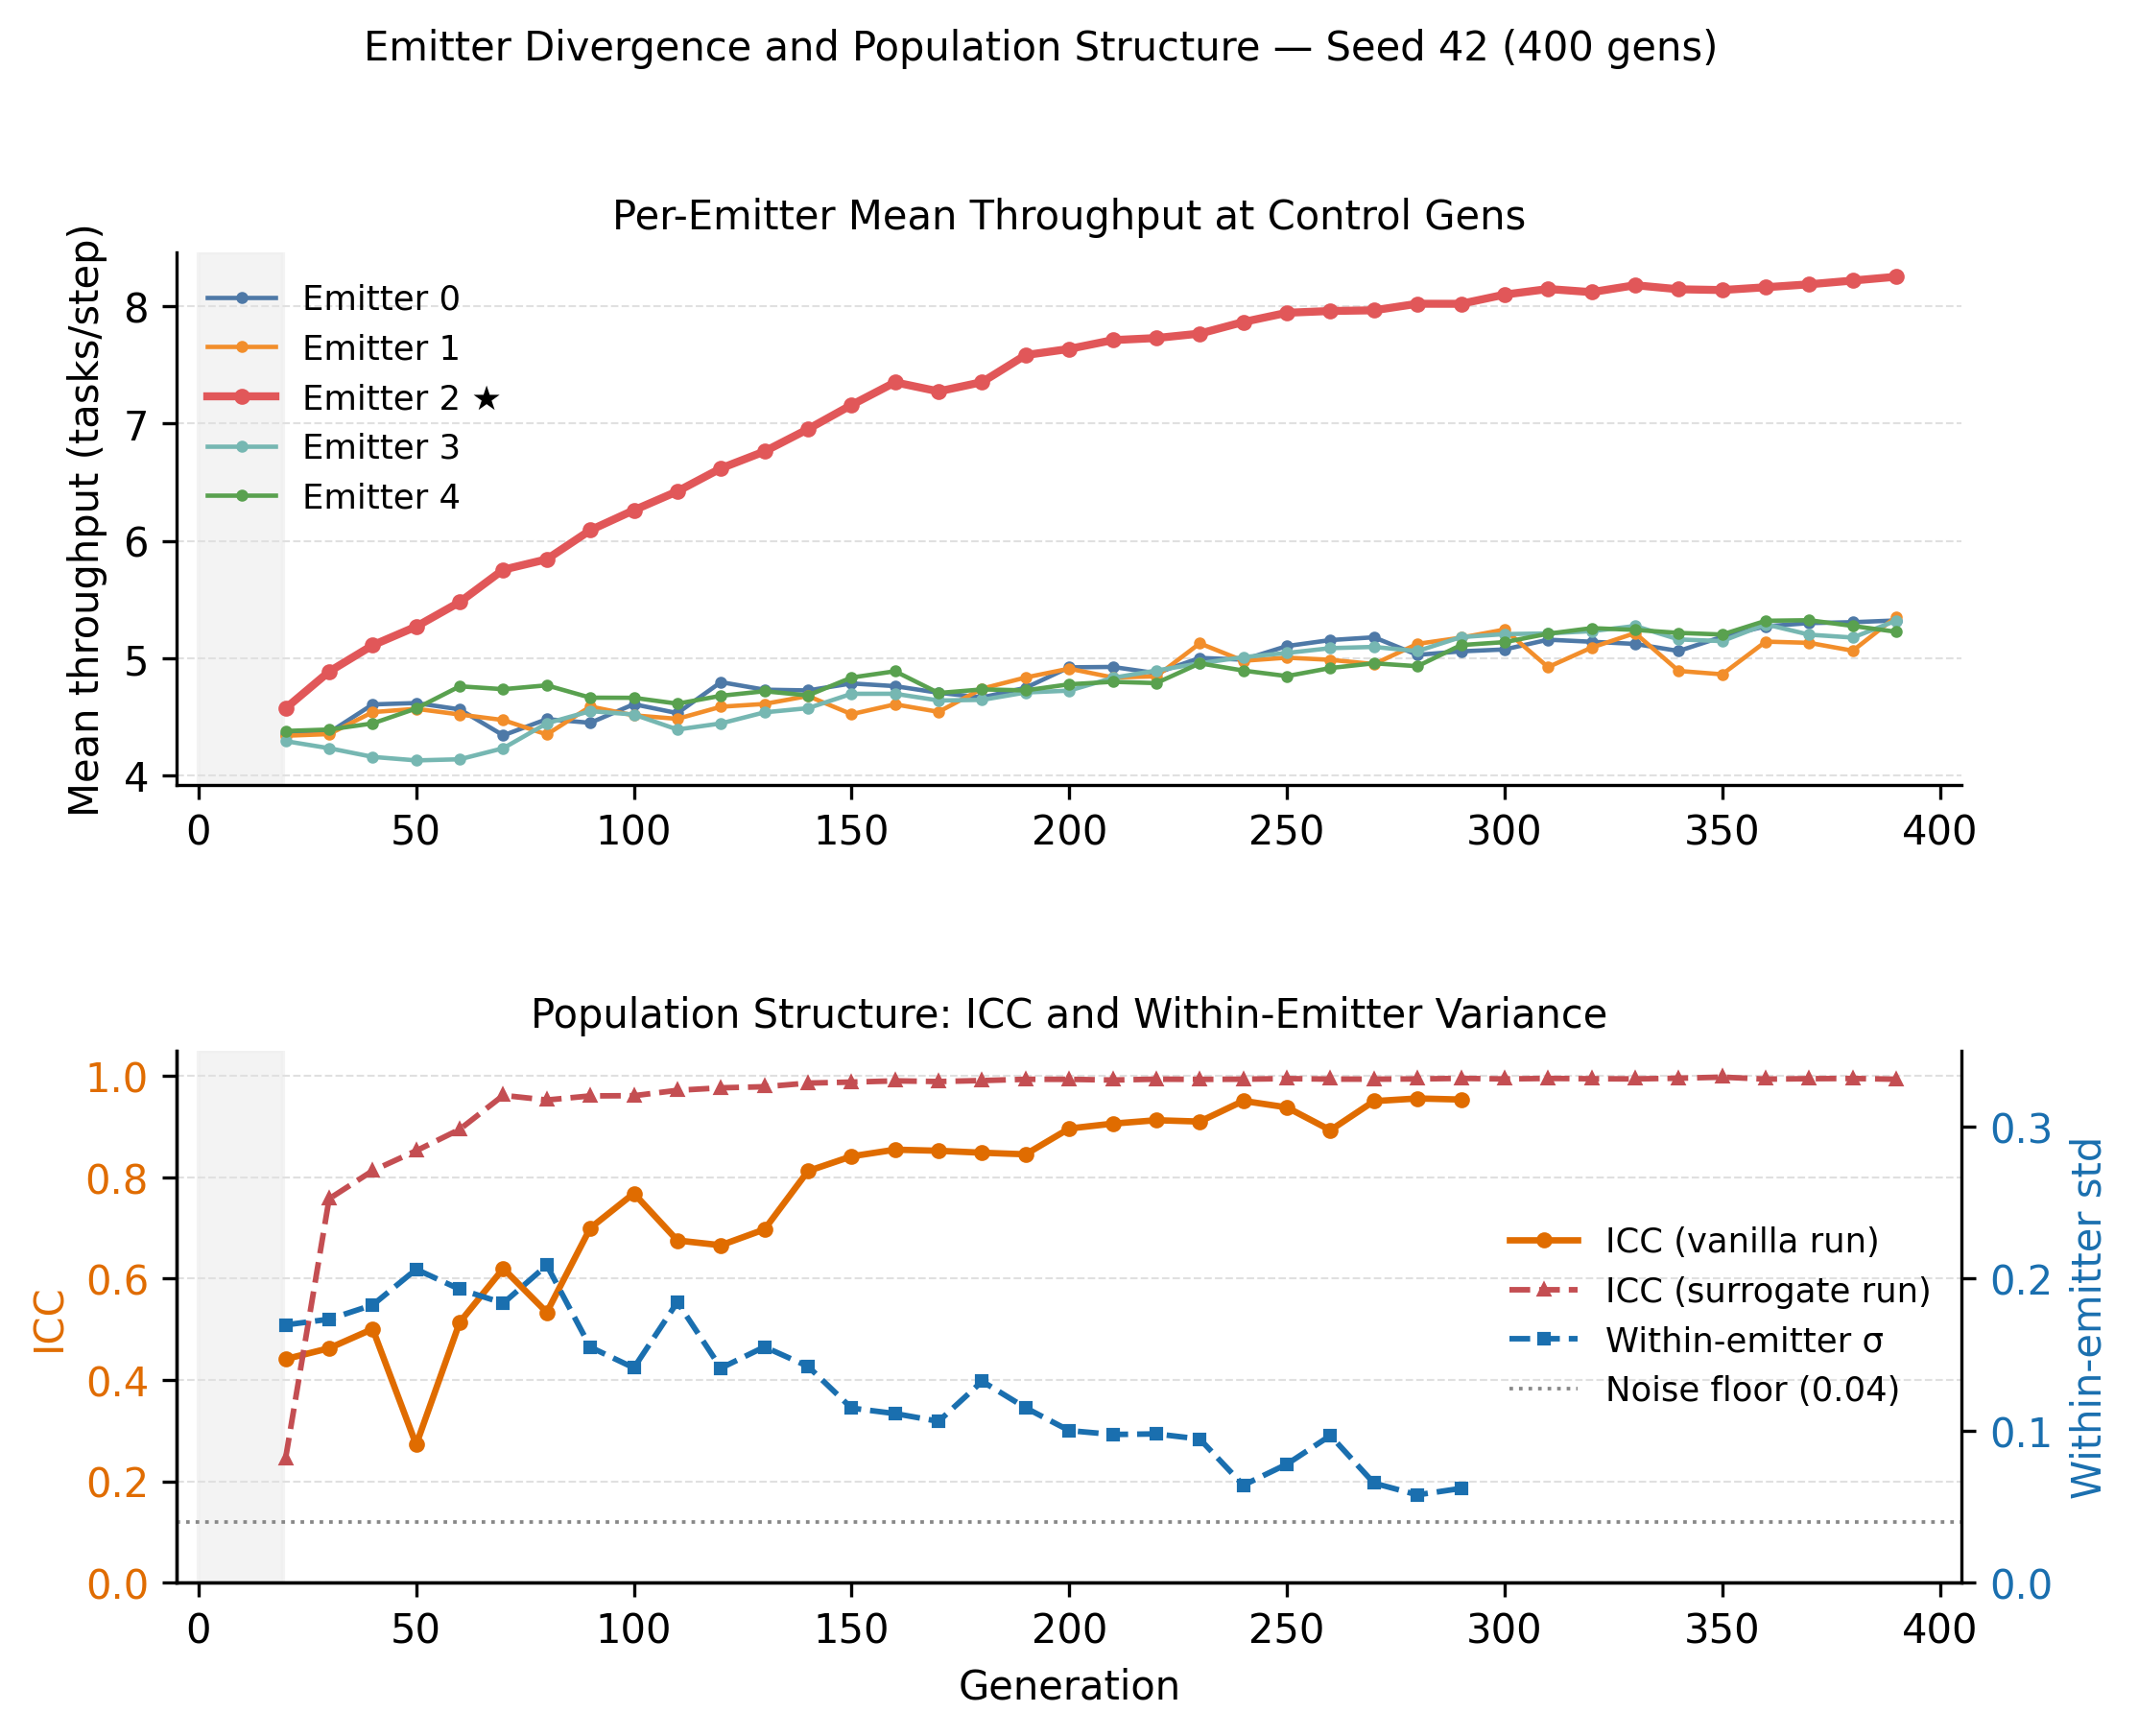
\includegraphics[width=0.48\textwidth]{fig11_rho_emitter_structure}}
  \caption{Top: per-emitter mean throughput at evolution control
           generations of the surrogate run. Emitter~2 (red) diverges
           to 8.22 by generation 380 while emitters 0, 1, 3, and 4
           plateau near 5.1 from generation 60.
           Bottom: ICC in the vanilla run (orange solid, left axis) and
           in the surrogate run (red dashed, left axis), with
           within-emitter standard deviation (blue, right axis).
           In the vanilla run ICC grows gradually from 0.44 to 0.95 as
           emitters diverge naturally; in the surrogate run ICC saturates
           near 1.0 by generation 40 because UCB screening reinforces
           emitter~2's dominance. Within-emitter $\sigma$ falls toward
           the measurement noise floor (dotted).}
  \label{fig:rho_emitter}
\end{figure}

The bottom panel of Fig.~\ref{fig:rho_emitter} shows ICC growing from
0.44 at generation 20 to 0.95 by generation 280 in the vanilla run
(orange solid).
In the surrogate run (red dashed), ICC saturates near 1.0 by generation
40: UCB screening concentrates simulations on emitter~2, reinforcing its
lead and driving between-emitter divergence far faster than natural
evolution alone.
Simultaneously, within-emitter $\sigma$ falls from 0.17 to 0.06,
approaching the measurement noise floor of 0.04.
At ICC $= 0.95$, a model that identifies which emitter a candidate
belongs to will rank 95\% of the population correctly - a coarse
task learnable even in a 4,074-dimensional space.
In practice this means the surrogate confidently separates emitter~2's
candidates from the rest, but with emitters 0, 1, 3, and 4 all producing
similar mean throughputs their 80 candidates are largely indistinguishable
from one another. This explains why overall $\rho$ sits near 0.60 rather
than approaching 1, and why it varies erratically across control
generations depending on how those four clusters happen to be sorted by
the model at each evaluation.
In the single-emitter setting, ICC $= 0$ by construction; the oracle
test confirms that the resulting fine-grained regression task is
infeasible due to landscape roughness.
To assess whether richer architectures overcome this, we evaluated
LargeCNN (five-layer 2-D CNN on the spatial weight tensor),
CellTransformer (per-cell attention over all 948 warehouse cells), and a
GAT-based GNN operating on the warehouse topology. All three produced
$\rho \approx 0$ in oracle mode; the best sliding-window result was
LargeCNN at median $\rho = 0.17$ (Table~\ref{tab:rho_comparison}), well
below the $\rho > 0.8$ generally required for reliable
screening~\cite{jin2011,hansen2019,akimoto2022}.
Within-emitter fine-grained ranking therefore appears infeasible
independent of model expressivity, and high ICC is a necessary condition
for surrogate-assisted CMA-ES.

\begin{table}[htbp]
  \caption{Spearman $\rho$ by population structure. Five-emitter values
           are from all evolution control generations of the V3 run.
           Single-emitter values are from the sliding-window temporal
           test; XGBoost, MLP, and simple CNN were evaluated across
           eight test generations and the remaining architectures across
           five.}
  \label{tab:rho_comparison}
  \begin{center}
    \begin{tabular}{lcc}
      \toprule
      \textbf{Condition} & \textbf{Median $\rho$} & \textbf{Range} \\
      \midrule
      Five-emitter (control gens) & 0.60 & 0.22--0.84 \\
      One-emitter, XGBoost        & 0.05 & 0.00--0.12 \\
      One-emitter, MLP            & 0.01 & $-$0.14--0.24 \\
      One-emitter, simple CNN     & 0.14 & $-$0.08--0.33 \\
      One-emitter, LargeCNN       & 0.17 & $-$0.04--0.42 \\
      One-emitter, CellTransformer & 0.08 & 0.02--0.21 \\
      One-emitter, GNN            & 0.03 & $-$0.07--0.16 \\
      \bottomrule
    \end{tabular}
  \end{center}
\end{table}

\subsection{Exploration Weight ($\lambda$) Ablation}

Table~\ref{tab:results} summarises all three configurations. The relationship
is non-monotone: $\lambda = 0$ (8.04) and $\lambda = 2.0$ (7.86) both
underperform $\lambda = 1.0$ (8.15). At $\lambda = 0$ the surrogate does not
evaluate candidates in newly-shifted emitter regions, leaving their CMA-ES
updates on stale predictions. At $\lambda = 2.0$ the uncertainty bonus
overrides the fitness signal too often, sending low-quality candidates to full
simulation. The quality differences across the three settings are modest and
based on a single run; the ablation confirms that some exploration weight is
preferable to none, but does not establish a precise optimal value.

\subsection{Online GGO Extension}
\label{sec:online}

Table~\ref{tab:online} summarizes the online GGO results. The surrogate
reduces the simulation count from 10,000 to 3,520, a 2.84x reduction.
A crossover-point analysis gives a precise picture: the vanilla run first
reaches a throughput of 7.332 at 8,300 cumulative simulations, while the
surrogate reaches the same quality at 3,440 simulations, a crossover
speedup of \textbf{2.41x}. Both runs are single executions; the 13.8-hour
per-run cost makes replication impractical within the scope of this work,
so this result should be treated as indicative.

\begin{table}[htbp]
  \caption{Online GGO Results (CNN Policy, 4,271 Parameters)}
  \label{tab:online}
  \begin{center}
    \begin{tabular}{lccc}
      \toprule
      \textbf{Method} & \textbf{Throughput} & \textbf{Simulations} & \textbf{Wallclock} \\
      \midrule
      Vanilla (online)            & 7.433 & 10,000 & 13.8\,h \\
      \textbf{Surrogate (online)} & \textbf{7.332} & \phantom{0}\textbf{3,520} & \textbf{4.9\,h} \\
      \bottomrule
    \end{tabular}
  \end{center}
\end{table}

The online surrogate $\rho$ behaved differently from the offline case.
Rank correlation was near zero for the first 50 generations (reaching as
low as $-0.167$ at generation 41), then improved sharply above generation
51, stabilizing at 0.55--0.71 for the remainder of the run. This phase
transition occurs because raw CNN parameter vectors do not have the smooth,
interpretable structure of static edge weight vectors. The MLP surrogate
requires approximately 1,800 real evaluations before it can learn useful
structure from the parameter space, compared to roughly 1,000 for the
offline case. Despite the poor early-phase accuracy, the surrogate still
delivered a 2.41x crossover speedup: the weak predictions in the early
phase did not derail the search, and the high-accuracy late phase
(generation 51--100) drove the final quality improvement from a throughput
of 6.21 to 7.33.

\begin{figure}[htbp]
  \centerline{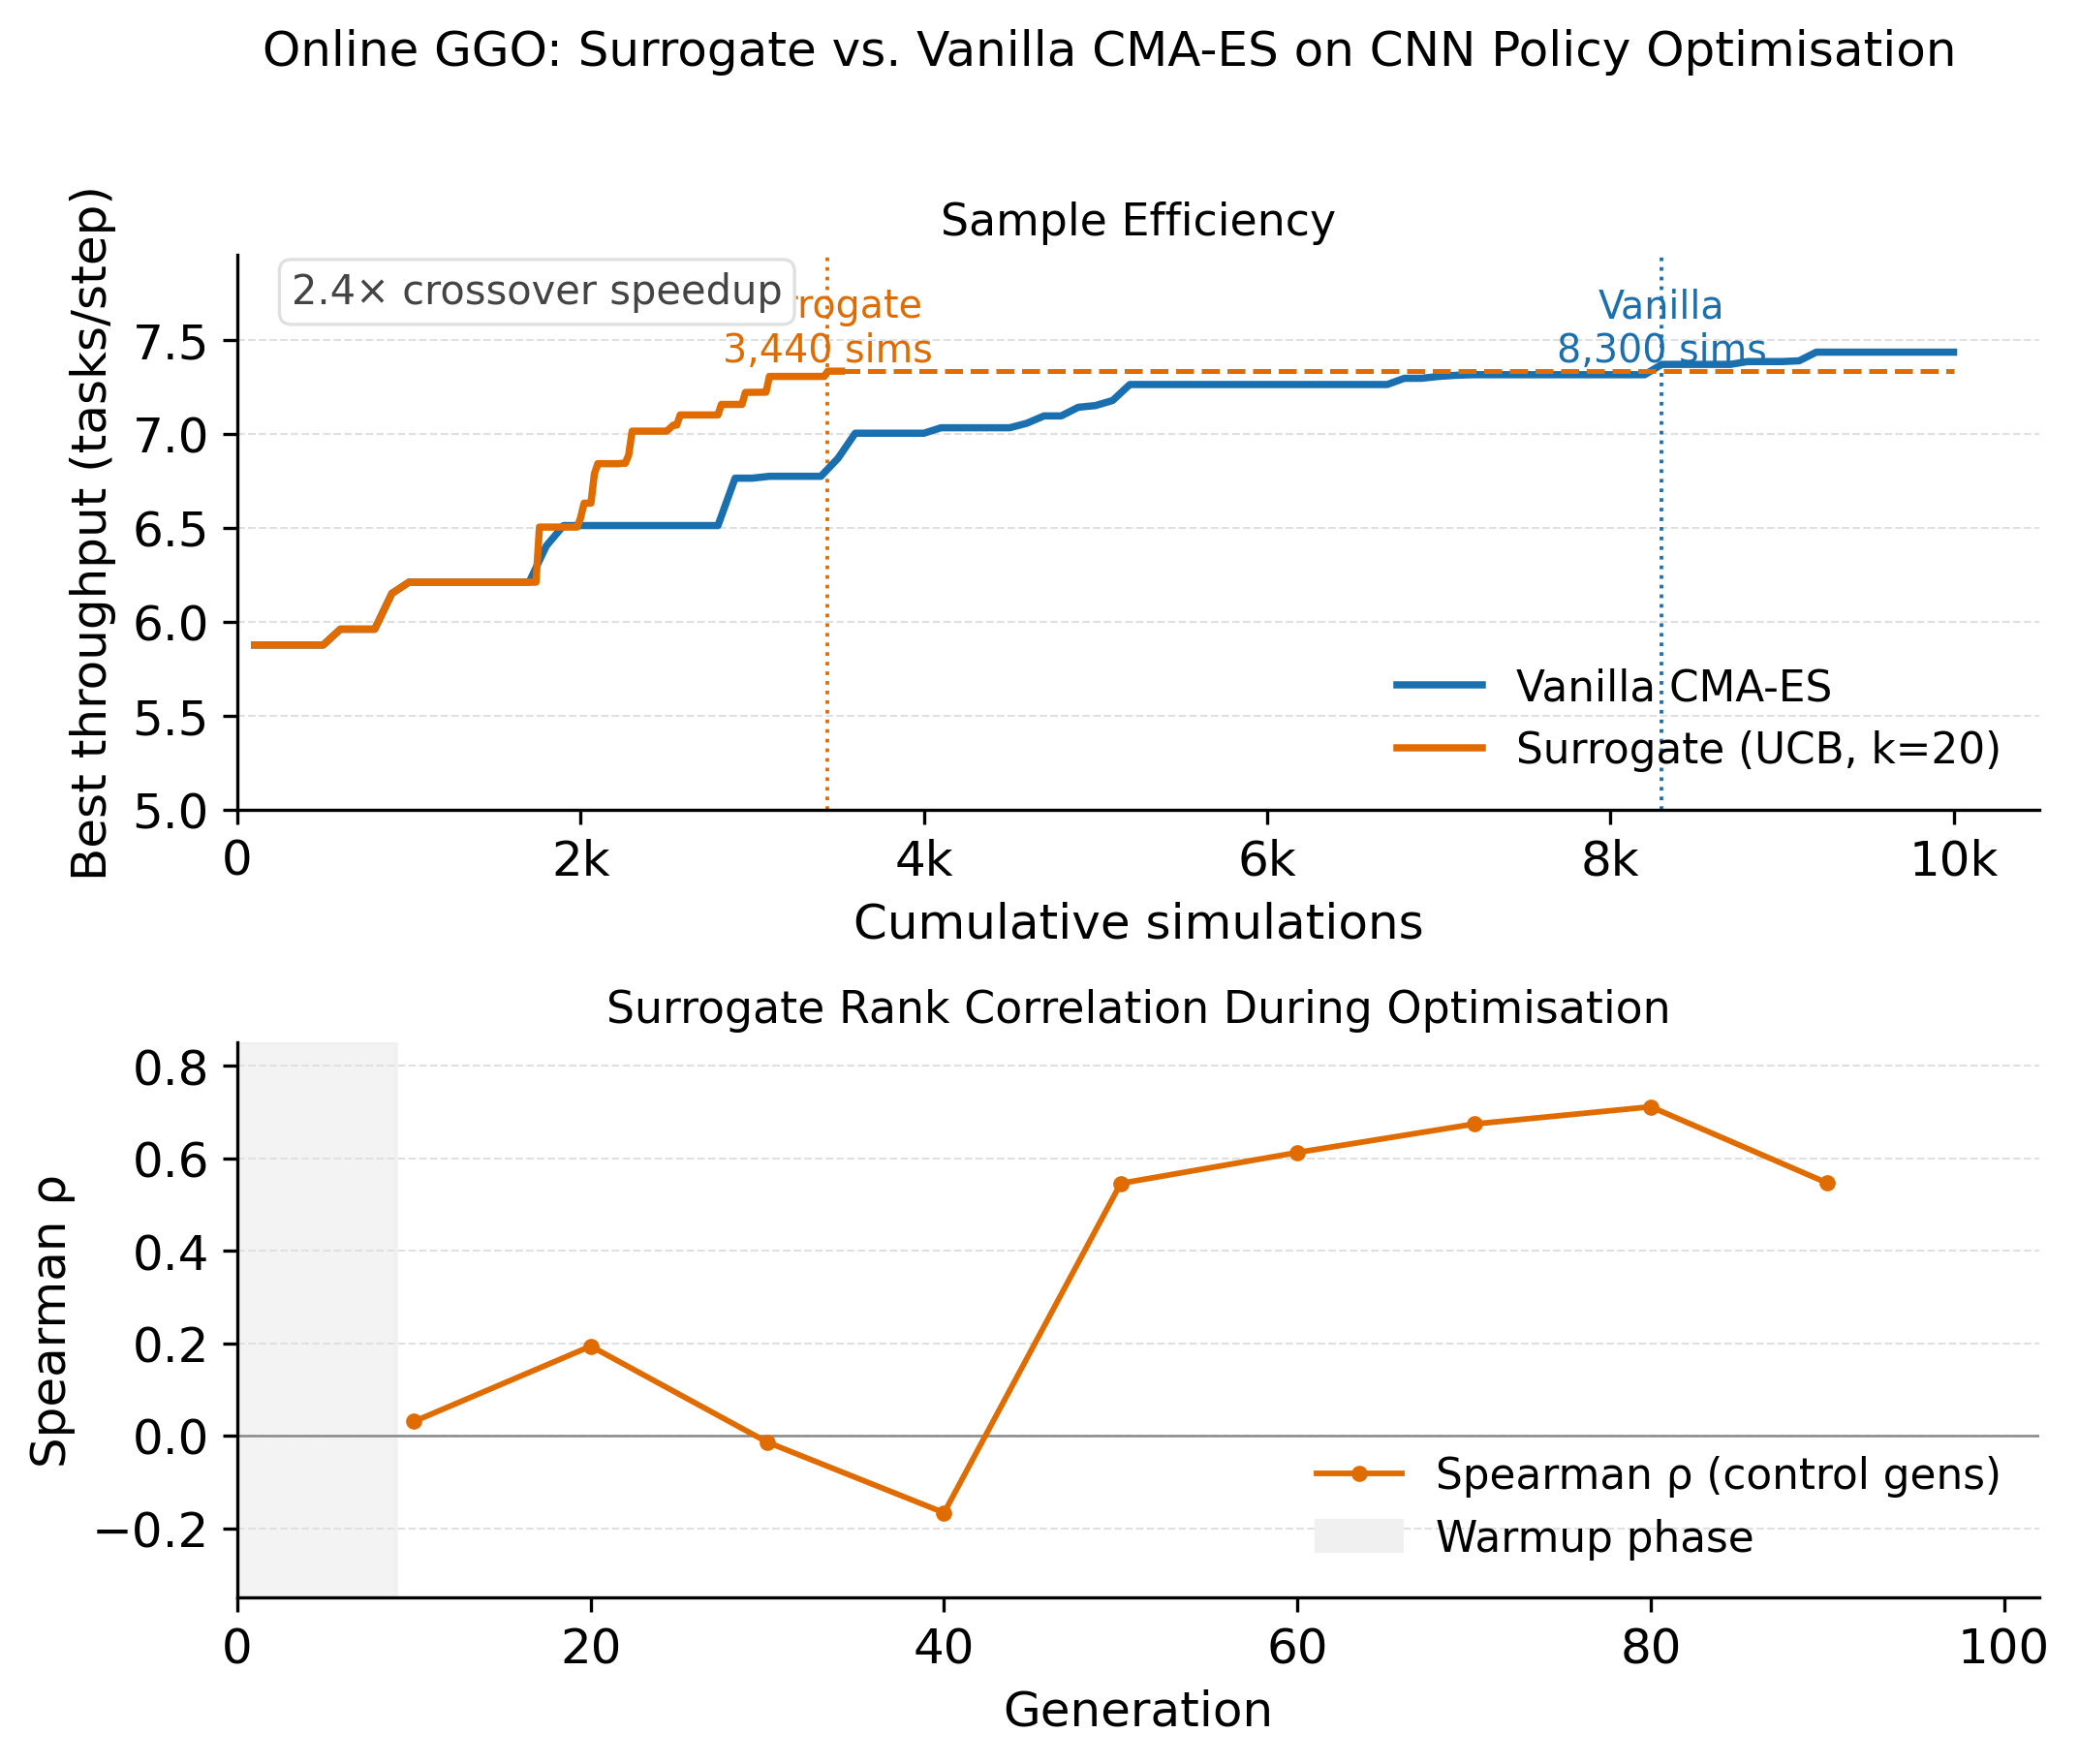
\includegraphics[width=0.48\textwidth]{fig7_online_ggo}}
  \caption{Online GGO extension. Top: sample efficiency in the online
           setting; the surrogate reaches the same quality as vanilla at
           2.41x fewer simulations. Bottom: surrogate rank correlation
           over 100 generations, showing a sharp phase transition near
           generation 51 once roughly 1,800 training samples have
           accumulated.}
  \label{fig:online}
\end{figure}


% ============================================================
%  7. DISCUSSION
% ============================================================

\section{Discussion}

\subsection{Why Ensemble UCB Closes the Throughput Gap}

V3 outperforms V1 because UCB sends candidates in newly-shifted emitter
regions to full simulation, keeping the CMA-ES update honest. V1 ranks
those candidates at random and corrupts the emitter update, a form of
surrogate exploitation that accumulates over multiple distribution shifts.
The quality difference between $\lambda=0$ and $\lambda=1.0$ is modest
(+1.4\% on corrected means) and from a single run; both surrogate variants
are outperformed on sample efficiency by a single-emitter CMA-ES without
any surrogate.


\subsection{Negative Result: Post-Hoc Gradient Refinement}

After the main experiments we tested whether gradient ascent through the
trained ensemble could improve the best solution found by V3. Starting from
the V3 best, we ran 1,000 gradient steps using the uncertainty-penalized
score $\mu - \lambda\sigma$ with L2 regularization
($\text{reg} = 10^{-6}$).

The surrogate predicted a gain of $+0.95$ (from 7.60 to 8.55). The actual
simulation showed a decrease of $-0.11$ from the V3 best (8.23 to 8.12).
Two problems compounded. First, the surrogate underestimated the V3 best
solution by 0.63 units at the starting point, showing poor calibration at
the high-quality region. Second, over 1,000 gradient steps the optimizer
moved $L_2 = 493$ units through solution space into a region where the
model overestimated by $+0.44$ units. The prediction error changed sign,
which is a direct sign of surrogate exploitation.

This confirms why V3 uses the surrogate conservatively. The UCB score
selects which of 100 CMA-ES-proposed candidates to evaluate; it never
requires the model to be accurate far from the training distribution.
Gradient ascent has no such constraint and can be led into regions where
model error is large. Direct gradient optimization through this surrogate
is not reliable in this setting.

\subsection{Population Structure as a Necessary Condition}

The ICC analysis in Section~\ref{sec:population_structure} has a direct
practical implication: offline feasibility studies conducted on
multi-emitter data will systematically overestimate live accuracy whenever
ICC in the offline dataset exceeds ICC during deployment. Surrogate-assisted
evolutionary algorithms should therefore be benchmarked under population
diversity conditions matching deployment, and ICC should be reported
alongside accuracy metrics as a predictor of whether surrogate
pre-screening will be effective.


% ============================================================
%  8. CONCLUSION AND FUTURE WORK
% ============================================================

\section{Conclusion and Future Work}

The central theoretical finding of this paper is that surrogate
pre-screening in multi-emitter CMA-ES is effective because the
population's intraclass correlation coefficient (ICC) grows high as
emitters diverge, reducing the surrogate's task from fine-grained fitness
regression to cluster identification. In the single-emitter case ICC is
zero by construction and the surrogate fails regardless of model capacity
or data volume, as confirmed by three escalating diagnostic tests. This
identifies ICC as a necessary condition for surrogate-assisted CMA-ES,
not merely an observed property of the runs.

Under this condition, surrogate-assisted evolutionary strategies
substantially reduce the computation required for LMAPF guidance graph
optimization. Replacing most simulations with ensemble MLP predictions
gives a 2.81x crossover speedup on the primary run: V3 reaches a
throughput of $\tau = 8.23$ using 49k simulations, while vanilla CMA-ES
requires 137k. A second warehouse seed (123) yields a consistent 2.92x
speedup, confirming the result is not seed-dependent. Vanilla ran for 300
generations and V3 for 400; V3's final score of 8.33 slightly exceeds
vanilla's 8.29, confirming the surrogate does not degrade solution quality.
The gradient refinement experiment gives a concrete example of surrogate
exploitation: the surrogate predicted a $+$0.95 gain but simulation
measured a $-$0.11 decrease. The conservative UCB design guards against
this failure mode and is recommended as a default for future surrogate
work in this setting; the ablation evidence for a specific optimal
$\lambda$ is from a single run and should be treated as indicative.

Robustness experiments on a second random seed and a different map type
confirm that the efficiency advantage generalises, with the caveat that
problems that converge before the warmup phase ends do not benefit from
screening.

We also show that the framework transfers to the online GGO setting of
Zang et al.~\cite{zang2025}, who called for exactly this type of work.
Applying the surrogate to a CNN guidance policy (4,271 parameters) reduces
simulation count from 10,000 to 3,520, reaching equivalent throughput
quality at a 2.41x crossover speedup. The online surrogate exhibits a
learning threshold at roughly 1,800 training samples, after which rank
correlation rises sharply from near zero to 0.55--0.71. This shows that
the surrogate framework generalizes across both static and adaptive
guidance representations, and that the required data volume scales with
the structural complexity of the search space.

\subsection{Limitations}

All offline experiments used a single warehouse map with a fixed agent
count and goal distribution; results on varied layouts, densities, or task
structures are unknown. The offline comparison covers two random seeds and
one additional map type, which is sufficient to rule out a single lucky
draw but not to characterize the full variance across environments. The
approach requires a multi-emitter configuration to achieve the population
diversity that makes surrogate pre-screening feasible (high ICC). To quantify how much of the efficiency gain comes from implicit emitter
selection rather than surrogate ranking, we ran a single-emitter baseline:
one CMA-ES instance with population size 100 and no surrogate. This baseline
reaches the same $\tau=8.23$ threshold at 41\,500 cumulative simulations, a
3.30x reduction relative to the 5-emitter vanilla run, which exceeds Surrogate
V3's 2.81x. The surrogate therefore does not outperform a simple single-emitter
run on this metric, and emitter starvation driven by UCB is the primary
mechanism behind the reported speedup. Finally, the online GGO comparison is a
single run of each method and should be treated as preliminary given the
13.8-hour per-run cost.
Among the architectures evaluated in the single-emitter diagnostic, only
LargeCNN offers training times compatible with the live surrogate loop;
CellTransformer and the graph neural network require substantially more
compute per generation and are not practical as drop-in replacements
without further optimisation.

The more productive research directions are alternative genotype
representations that expose smoother fitness landscape structure and
feature engineering that encodes warehouse graph topology into the
surrogate input. If either raises within-emitter rank correlation above
the screening threshold, LargeCNN is the most practical starting
architecture given its compatible training times.

% ============================================================
%  ACKNOWLEDGMENT
% ============================================================

\section*{Acknowledgment}

The author thanks Prof. Gerhard Weiss for guidance throughout this project
and the Department of Advanced Computing Sciences at Maastricht University
for providing computing resources.

% ============================================================
%  REFERENCES
% ============================================================

\begin{thebibliography}{00}

\bibitem{zhang2024}
J.~Zhang, Y.~Jiang, V.~Bhatt, S.~Nikolaidis, and J.~Li,
``Guidance graph optimization for lifelong multi-agent path finding,''
in \textit{Proc. Int. Joint Conf. Artificial Intelligence (IJCAI)},
pp.~311--320, 2024.

\bibitem{zang2025}
H.~Zang, Y.~Zhang, H.~Jiang, Z.~Chen, D.~Harabor, P.~J.~Stuckey,
and J.~Li, ``Online guidance graph optimization for lifelong
multi-agent path finding,'' in \textit{Proc. AAAI Conf. Artificial
Intelligence (AAAI)}, pp.~14726--14735, 2025.

\bibitem{jin2011}
Y.~Jin, ``Surrogate-assisted evolutionary computation: Recent advances and
future challenges,'' \textit{Swarm and Evolutionary Computation}, vol.~1,
no.~2, pp.~61--70, 2011.

\bibitem{hansen2019}
N.~Hansen, ``A global surrogate assisted {CMA-ES},'' in \textit{Proc.
Genetic and Evolutionary Computation Conference (GECCO)}, pp.~664--672,
2019.

\bibitem{akimoto2022}
Y.~Akimoto, A.~Miyagi, and J.~Sakuma, ``Analysis of surrogate-assisted
information-geometric optimization algorithms,'' \textit{Algorithmica},
vol.~85, pp.~1--38, 2022.

\bibitem{auer2002}
P.~Auer, N.~Cesa-Bianchi, and P.~Fischer, ``Finite-time analysis of the
multiarmed bandit problem,'' \textit{Machine Learning}, vol.~47,
no.~2--3, pp.~235--256, 2002.

\bibitem{shahriari2016}
B.~Shahriari, K.~Swersky, Z.~Wang, R.~P.~Adams, and N.~de Freitas,
``Taking the human out of the loop: A review of Bayesian optimization,''
\textit{Proc. IEEE}, vol.~104, no.~1, pp.~148--175, 2016.

\bibitem{hansen2016}
N.~Hansen, ``The CMA evolution strategy: A tutorial,''
\textit{arXiv preprint arXiv:1604.00772}, 2016.

\bibitem{lakshminarayanan2017}
B.~Lakshminarayanan, A.~Pritzel, and C.~Blundell,
``Simple and scalable predictive uncertainty estimation using deep
ensembles,'' in \textit{Proc. Advances in Neural Information Processing
Systems (NeurIPS)}, pp.~6402--6413, 2017.

\bibitem{spearman1904}
C.~Spearman, ``The proof and measurement of association between two things,''
\textit{American Journal of Psychology}, vol.~15, pp.~72--101, 1904.

\bibitem{shrout1979}
P.~E.~Shrout and J.~L.~Fleiss, ``Intraclass correlations: Uses in
assessing rater reliability,'' \textit{Psychological Bulletin},
vol.~86, no.~2, pp.~420--428, 1979.

\bibitem{fontaine2020}
M.~C.~Fontaine, J.~Togelius, S.~Nikolaidis, and A.~K.~Hoover,
``Covariance matrix adaptation for the rapid illumination of behavior
space,'' in \textit{Proc. Genetic and Evolutionary Computation
Conference (GECCO)}, pp.~94--102, 2020.

\end{thebibliography}

\end{document}